\documentclass[11pt]{article}
\usepackage[T1]{fontenc}
\usepackage[margin=1in]{geometry}
\usepackage{amsmath,amssymb,amsthm}
\usepackage{graphicx}
\usepackage[colorlinks=true,linkcolor=blue,citecolor=blue,urlcolor=blue]{hyperref}
\newtheorem{lemma}{Lemma}[section]
\newtheorem{proposition}[lemma]{Proposition}
\theoremstyle{remark}
\newtheorem{remark}[lemma]{Remark}
\newcommand{\Tr}{\operatorname{Tr}}

\title{CMI-Based Recoverability versus Wilson-Loop Diagnostics in
$\mathbb{Z}_2$ Lattice Gauge Theory (2+1D)\\
{\large Exact diagonalization benchmark on small open lattices}\\
{\normalsize Version 2}}
\author{Lluis Eriksson\\ Independent Researcher\\ \texttt{lluiseriksson@gmail.com}}
\date{January 2026 (v1); July 2026 (v2)}

\begin{document}
\maketitle

\begin{abstract}
We provide a finite-size benchmark testing whether a CMI-based
recoverability proxy correlates with Wilson-loop confinement diagnostics
in $\mathbb{Z}_2$ lattice gauge theory in 2+1 dimensions, computing ground
states by sparse exact diagonalization on $2\times2$ and $2\times3$ open
lattices (link qubits, Gauss-law penalty verified by $\langle G_v\rangle
\simeq 1$) and evaluating entropic quantities by pure-state Schmidt/SVD.
We state a conditional bridge from a spatial area law to an operational
``information horizon'' via explicit hypotheses (H1)--(H4), with two
recovery-length conventions (absolute, and normalized by the boundary
prefactor $\Sigma_B(w) = |\partial B(w)|\log 2$). \emph{v2 (no v1 number
is changed) adds a structural lemma that v1's own Table 1 was exhibiting
unnoticed:} for a pure global state, when the collar saturates
($B = (A\cup C)^c$) purity forces $I(A{:}C|B) = I(A{:}C|\emptyset)$ --
this is exactly why v1's Table 1 shows $I(w{=}2) = I(w{=}0) = 0.4992999$
to seven digits; the saturated row carries no buffer information, and the
informative range of that benchmark is $w \in \{0, 1\}$. v2 also anchors
the non-monotonicity of CMI under collar enlargement as
geometry-dependent (v1's wall geometry shows growth at $w{=}0 \to 1$; a
BFS-patch geometry on the same states decays monotonically -- there is no
data-processing theorem in that direction); cross-links the CMI benchmark
to the Petz-error twin on the same lattices (densified $n = 8$ sweep:
Spearman rank-trend $+1.00$, permutation $p = 10^{-4}$, against both
$1/\sigma_{\rm eff}$ \emph{and} the inverse spectral gap -- so, as in the
twin, confinement specificity is unresolved at these sizes); harmonizes
the fidelity convention (v1 correctly uses root fidelity with
$I \ge -2\log f$, equivalent to the companions' squared-convention
$I \ge -\log F$); removes an internal phase label leaked into v1's
Section 1 title and a duplicated heading; and adds series positioning and
a regenerable verification suite. The conditional proposition and its
hypotheses are unchanged.
\end{abstract}

\section{Conditional bridge: confinement as an information horizon}
As in v1 (unchanged; the internal phase label in the v1 heading is
removed and the duplicated subsection title merged): transfer-matrix
state $\rho_{\beta_T}$ (or ground-state limit); spatial Wilson loops and
spatial string tension $\sigma_{\rm str}$ with finite-size Creutz proxies
on small lattices; tripartition with collar $B(w)$ and boundary prefactor
$\Sigma_B(w) = |\partial B(w)|\log 2$; CMI in nats; absolute and
normalized recovery lengths $\xi^{\rm abs}_{\rm rec}(\varepsilon)$,
$\xi^{\rm norm}_{\rm rec}(\varepsilon)$; hypotheses (H1) spatial area
law, (H2) wall geometry forces $\mathrm{Area}_{\min}(w) \ge c_0 w$,
(H3$_g$) flux-tube-dominated exponential suppression of loop-restricted
connected leakage $\Delta_{\rm loop}(w)$, (H4$_{\rm QI}$) structural
leakage-to-CMI input; and the conditional proposition
$I(A{:}C|B(w)) \le K\,\Sigma_B(w)\,e^{-\alpha w}$ with
$\alpha = p\kappa\sigma_{\rm str}c_0$, $K = K_I C_f K_\Delta^p$, plus the
recovery corollary. \emph{Convention note (added in v2):} v1 states the
Fawzi--Renner corollary with root fidelity $F = \|\sqrt\rho\sqrt\sigma
\|_1$ and $I \ge -2\log F$ -- which is correct; the companions use the
squared convention with $I \ge -\log F^2$-equivalently. The identity
$-2\log f = -\log(f^2)$ makes both the same statement (suite-checked);
we flag it because this factor has historically been the most
error-prone convention point of the series.

\section{Saturation lemma and the informative range (added in v2)}
\begin{lemma}[Saturation identity]
\label{lem:sat}
Let $\rho_{\Lambda}$ be pure on a finite slice and let $A, C$ be disjoint
with $B := (A \cup C)^c$. Then
\[
I(A{:}C \,|\, B) \;=\; I(A{:}C \,|\, \emptyset) \;=\;
S(A) + S(C) - S(AC).
\]
\end{lemma}
\begin{proof}
Purity gives $S(AB) = S(C)$, $S(BC) = S(A)$ and $S(B) = S(AC)$, and
$S(ABC) = 0$; substitute into the CMI definition.
(Machine-verified on random pure states and on the $\mathbb{Z}_2$ ground
state, errors $\sim 10^{-15}$.)
\end{proof}
\begin{remark}[Consequence for v1's Table 1]
\label{rem:table}
v1's wall-geometry table on the $2\times3$ lattice at $g = 0.5$ reports
$I(w{=}0) = 0.4992999$, $I(w{=}1) = 0.8974278$, $I(w{=}2) = 0.4992999$:
the exact seven-digit return at $w = 2$ is Lemma~\ref{lem:sat} in action
-- at $w = 2$ the wall exhausts the complement of $A \cup C$. By v1's own
pre-saturation definition that row should be excluded; the informative
range of the benchmark instance is $w \in \{0, 1\}$. All v1 numbers
stand; what changes is their reading.
\end{remark}
\begin{remark}[Non-monotonicity is geometry-dependent]
\label{rem:mono}
There is no data-processing theorem for enlarging the conditioning
system, so $I(A{:}C|B(w))$ need not decrease in $w$: v1's wall geometry
indeed grows from $w = 0$ to $1$ ($0.499 \to 0.897$). On the same class
of states, the BFS-patch geometry of the Petz twin decays monotonically
across the full coupling sweep (suite: $0/8$ growth instances). Collar
monotonicity is thus a property of the collaring rule (cf.\ the
collaring-rule framework of 2601.0043), not of CMI itself.
\end{remark}

\section{ED benchmark and cross-link to the Petz twin (upgraded in v2)}
The v1 wall-geometry instance (Table 1, Figures) stands unchanged. v2
adds the coupling-resolved benchmark on the $2\times2$ lattice with the
BFS-patch geometry shared with the Petz twin 2601.0047: over $n = 8$
couplings $g \in [0.5, 2.5]$, $I(A{:}C|B(1))$ falls monotonically from
$1.6\times10^{-4}$ to $1.8\times10^{-11}$ while $1/\sigma_{\rm eff}$
falls and the spectral gap grows; the Spearman rank-trend of
$I(A{:}C|B(1))$ against $1/\sigma_{\rm eff}$ is $+1.00$ (permutation
$p = 10^{-4}$) -- \emph{and equally} $+1.00$ against the inverse gap. As
in the twin, the CMI benchmark therefore shows a robust monotone
rank-trend in the deterministic coupling sweep whose confinement
specificity is unresolved at these sizes (the permutation $p$ quantifies
ordering strength, not statistical independence). The Petz-error and CMI
observables thus tell one consistent story on these lattices.

\begin{figure}[h]\centering
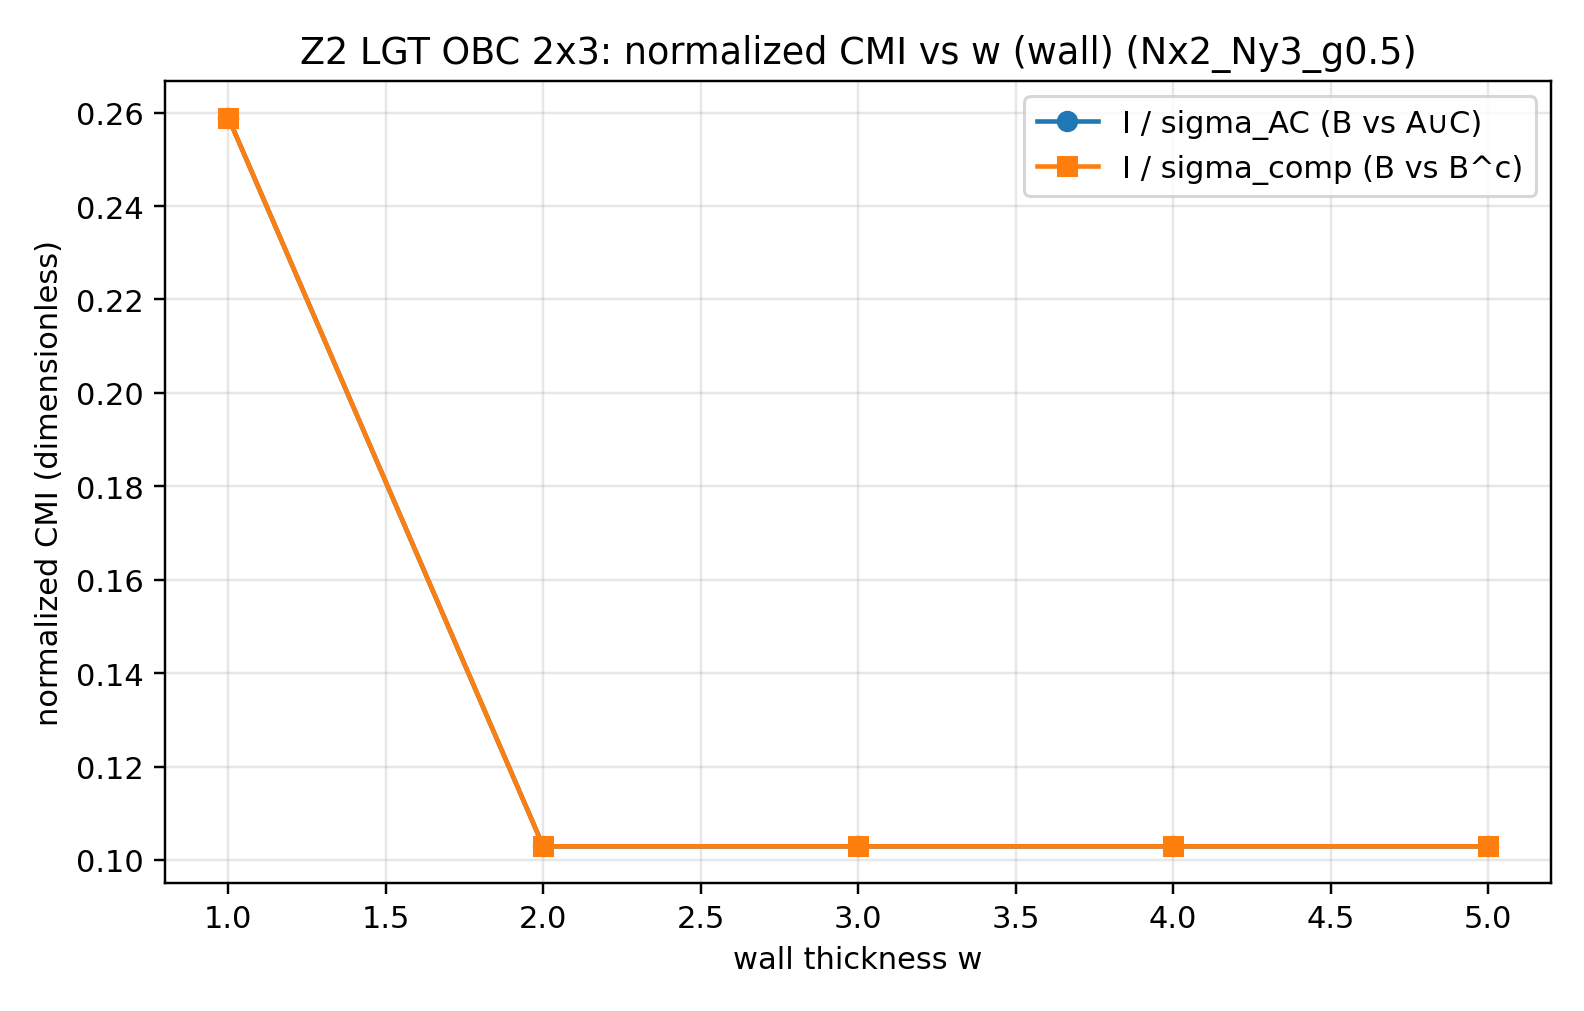
\includegraphics[width=0.48\textwidth]{fig1.png}
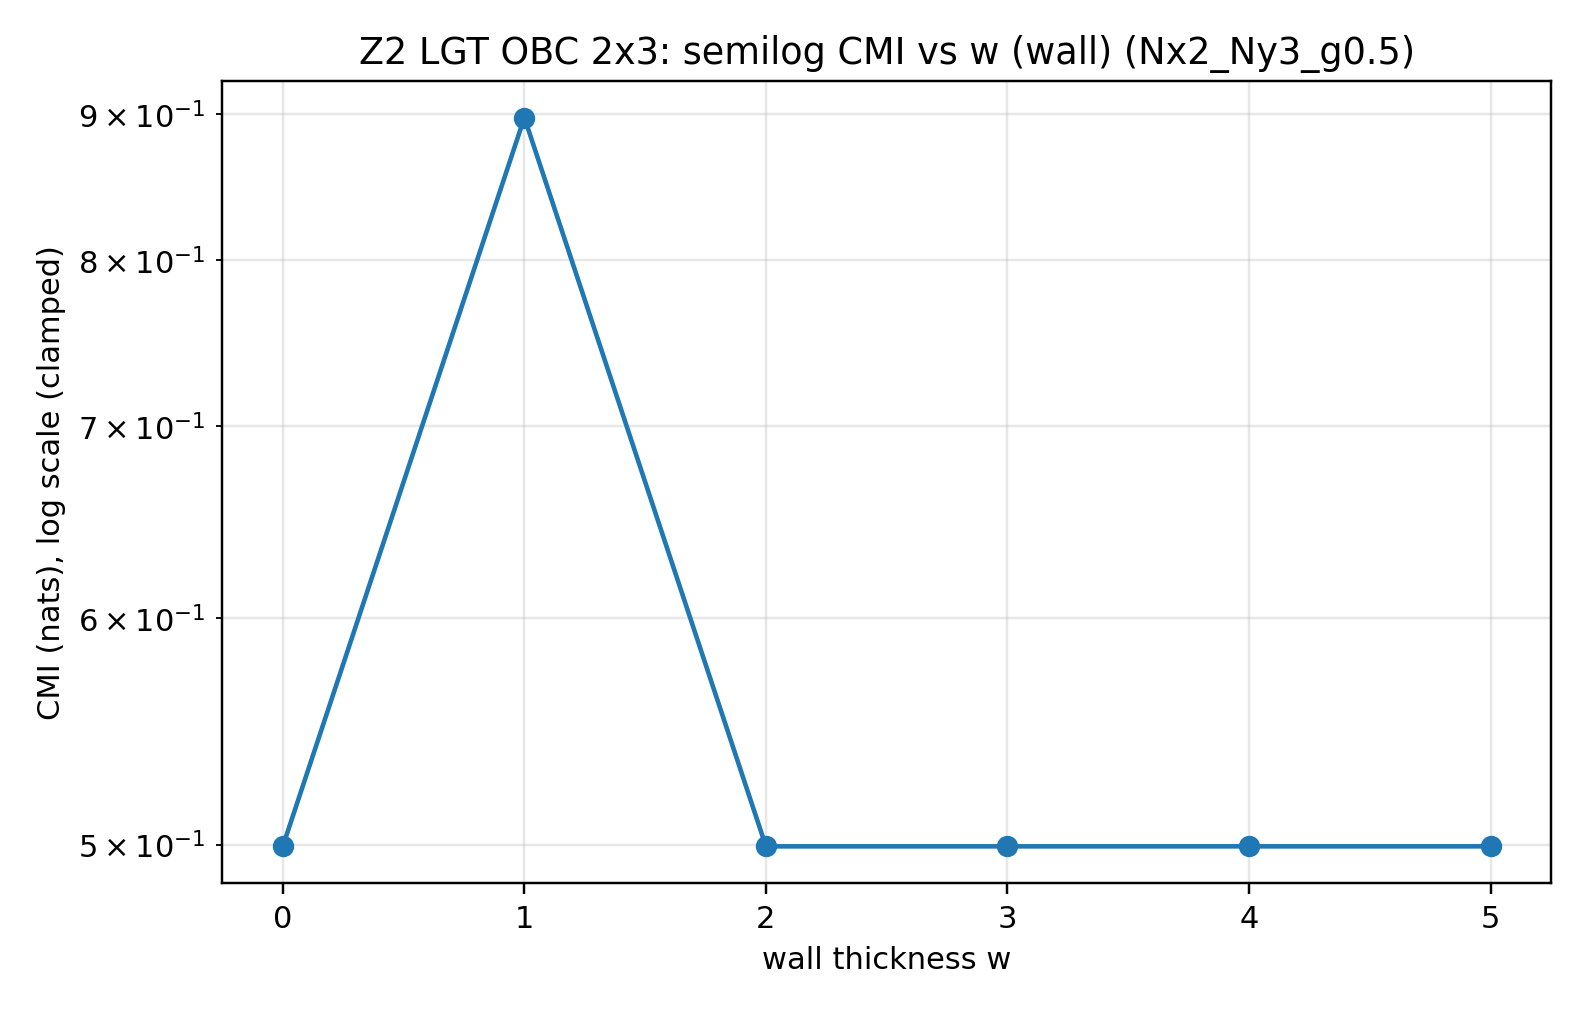
\includegraphics[width=0.48\textwidth]{fig2.png}
\caption{v1 wall-collar benchmark figures (unchanged): $I/\Sigma_B$ vs
$w$ and semilog $I$ vs $w$, $2\times3$, $g = 0.5$. Read with
Remarks~\ref{rem:table}--\ref{rem:mono}.}
\end{figure}

\section{Verification suite (added in v2)}
\texttt{verification/2601-0050/verify\_2601\_0050.py} (sparse Lanczos,
SVD entropies, chunked JSON cache): the saturation lemma on random pure
states and on the $\mathbb{Z}_2$ ground state (machine precision); the
geometry-dependence of collar monotonicity; the $n = 8$ CMI benchmark
with rank statistics and the gap covariate; Gauss-sector checks; and the
root/squared fidelity-convention identity.

\section{Discussion}
The conditional information-horizon proposition and its hypotheses are
untouched: (H4$_{\rm QI}$) remains the structural frontier, and the
uniformity-under-refinement remark remains the roadmap link to
recovery-based renormalization. What v2 contributes is discipline around
the benchmark: saturated rows are identities, collar monotonicity is a
collaring-rule property, the CMI and Petz-error twins agree, and the
confinement-vs-gap degeneracy identified in 2601.0047 v2 applies verbatim
here. Next steps are those of the twin: larger lattices, fixed-coupling
geometry sweeps, and sector-wise algebraic prescriptions.

\section*{Note added in v2}
No v1 number, hypothesis or proposition is changed. v2 adds: (1) the
saturation lemma (Lemma~\ref{lem:sat}) explaining Table 1's exact
$I(w{=}2) = I(w{=}0)$ coincidence and restricting the informative range
to $w \in \{0,1\}$; (2) the geometry-dependence of collar monotonicity
(Remark~\ref{rem:mono}); (3) the coupling-resolved CMI benchmark
cross-linked to 2601.0047 v2, with identical conclusions including the
unresolved confinement specificity; (4) the fidelity-convention
harmonization note (v1's root-fidelity factor is correct); (5) editorial
fixes: internal phase label removed from the Section 1 title, duplicated
heading merged; (6) series positioning (v1 cited no companion papers)
and the regenerable verification suite.

\begin{thebibliography}{10}
\bibitem{Kogut} J. B. Kogut, Rev. Mod. Phys. \textbf{51} (1979)
659--713.
\bibitem{Petz} D. Petz, Commun. Math. Phys. \textbf{105} (1986)
123--131.
\bibitem{FR} O. Fawzi and R. Renner, Commun. Math. Phys. \textbf{340}
(2015) 575--611.
\bibitem{S0047} L. Eriksson, ai.viXra:2601.0047 (2026; v2 2026).
\bibitem{S0044} L. Eriksson, ai.viXra:2601.0044 (2026; v2 2026).
\bibitem{S0046} L. Eriksson, ai.viXra:2601.0046 (2026; v2 2026).
\bibitem{S0043} L. Eriksson, ai.viXra:2601.0043 (2026; v2 2026).
\bibitem{S0020} L. Eriksson, ai.viXra:2601.0020 (2026; v2 2026).
\bibitem{S0035} L. Eriksson, ai.viXra:2601.0035 (2026; v2 2026).
\end{thebibliography}
\end{document}
